\section{Problem D}
\subsection{Task 1 and 2}

As we are trying to fit a normal distribution over the normalized proposed density function, the normal distribution must be scaled by a factor c so that it is larger than the proposed distribution for all values in the domain. This was done by numerically finding the maximum value of the proposed distribution. 

\begin{lstlisting}
y1 = 125
y2 = 18
y3 = 20
y4 = 34

theoretical_dist <- function(theta){
  return ((2+theta)^y1*(1-theta)^(y2+y3)*theta^y4)
}
max = optimize(theoretical_dist,interval = c(0,1),maximum = TRUE)
c = max$objective
\end{lstlisting}

C is evaluated to be: "1.838839e+29"

N samples from the distribution were generated with rejection sampling shown in the following code.

\begin{lstlisting}
samples = numeric()
steps = 0

n=10000
while (length(samples)<n){
  steps = steps+1
  
  x = rbeta(1,1,1);
  u = runif(1)
  alpha = (1/c)*(2+x)^y1*(1-x)^(y2+y3)*x^y4
  if(u<alpha){
    samples = c(samples,x)
  }
}
\end{lstlisting}

The posterior mean was simply calculated as

\begin{lstlisting}
    posteriori_mean = sum(samples)/n
\end{lstlisting}

The theoretical mean was calculated for comparison


\begin{lstlisting}
    normalize_const = integrate(theoretical_dist,0,1)
    
    #The theoretical density distribution multiplied by theta. 
    #The integral of this function produces the expected value.
    theta_times_dist <- function(theta){
        return ((2+theta)^y1*(1-theta)^(y2+y3)*theta^(y4+1))
    }

    theoretical_mean_non_norm = integrate(theta_times_dist,0,1)
    theoretical_mean = theoretical_mean_non_norm$value / normalize_const$value
\end{lstlisting}

The posteriori mean was calculated to be: 0.6230259
And the theoretical mean: 0.6228061
This verifies the calculation of the mean.

The histogram was then generated, and the theoretical normalized density was superimposed on the histogram. The result of this code is presented in figure \ref{fig:PD2_histogram}. This verifies that the distribution is correctly generated.
\begin{lstlisting}
    hist(samples,probability = TRUE)
    abline(v=posteriori_mean, col="red")
    
    x_real= (0:100)/100
    y_real = (1/normalize_const$value) * theoretical_dist(x_real)
    lines(x_real,y_real)
\end{lstlisting}

\begin{figure}[h!]
    \centering
    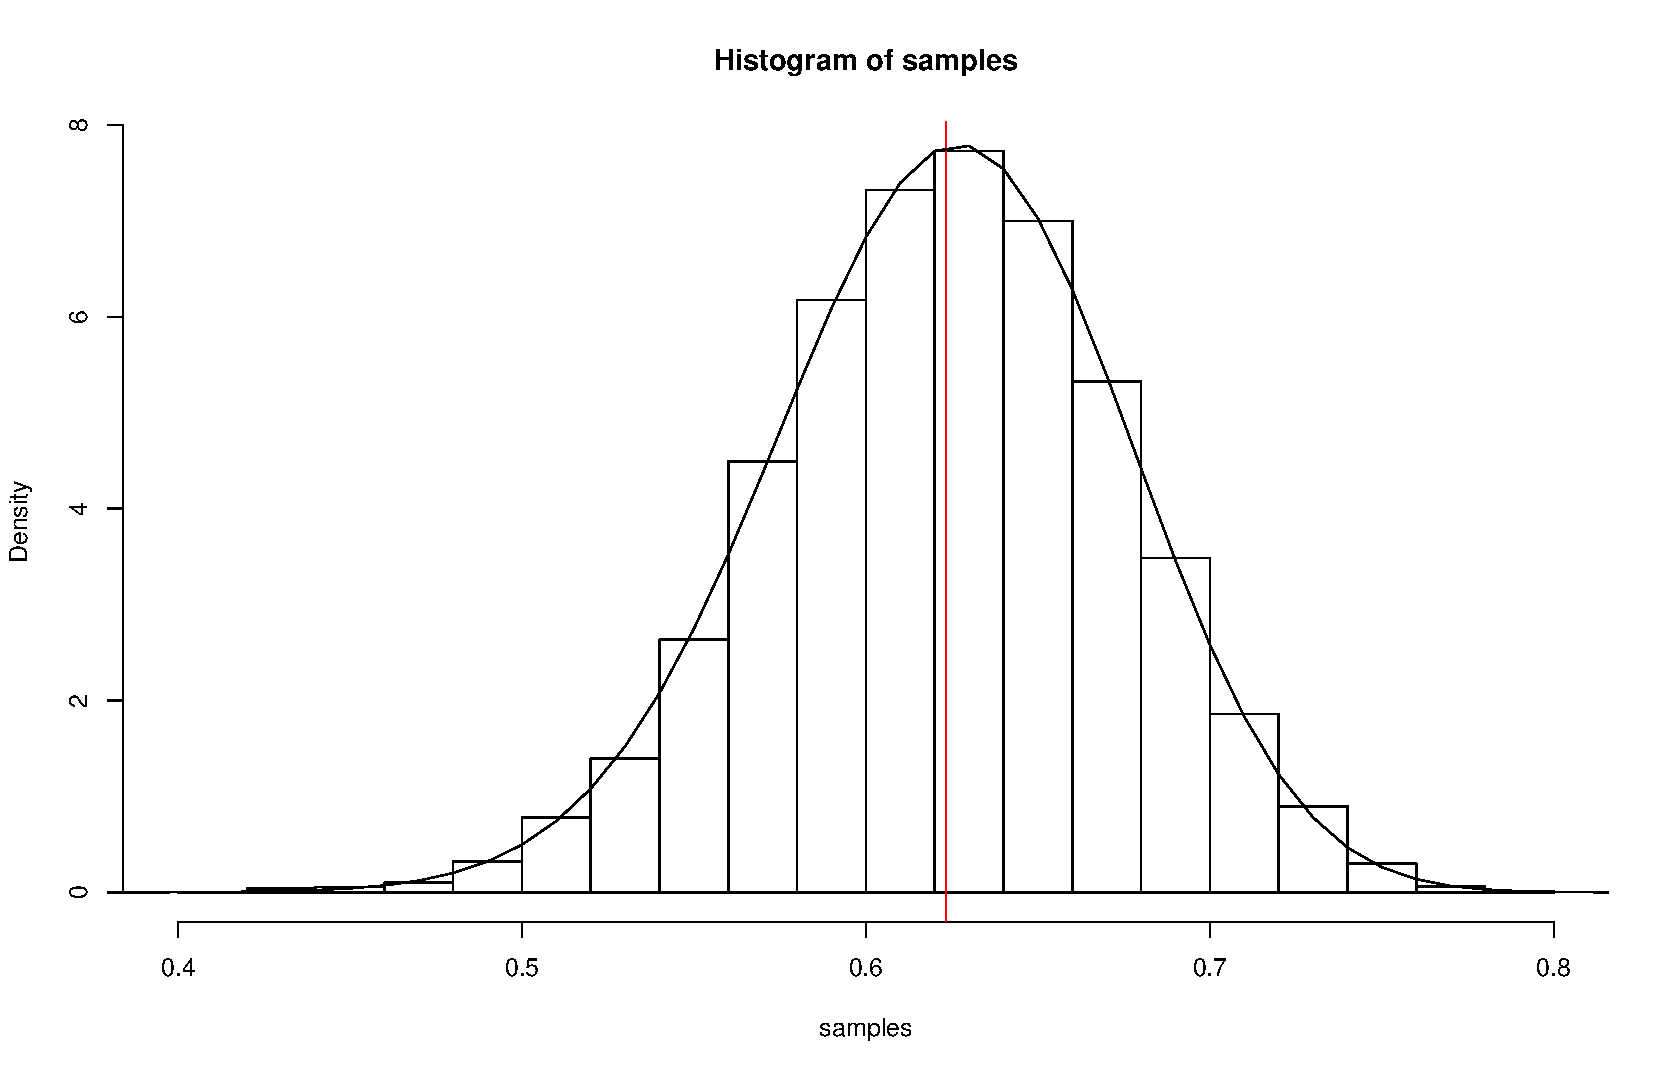
\includegraphics[width=\textwidth]{Ov1_D2_hist}
    \caption{HIstogram of 10000 samples produced with the density function proposed in task D. The true PDF is superimposed on the histogram. The red line shows the empirical posterior mean.}
    \label{fig:PD2_histogram}
\end{figure}

\subsection{Task 3}

The average number of samples needed per sample of the correct distribution with the rejection algorithm would be the ratio of the area between the scaled uniform distribution and the correct distribution. The area of the scaled unifrom distribution (on the interval 0-1) is simply the scaling constant c. The area of the normalized density function is the normalization constant. The theoretical average number of draws per accepted draw is then c divided by the normalization constant which evaluates to: 7.799308

The empirical average number of samples per correct can be calculated by dividing the number of steps the for rejection sampling for loop takes divided by the number of samples, n. This evaluates to: 7.7045

This verifies the theoretical result.

\subsection{4}

Previously we generated samples from the proposed multinomial mass function with a uniform prior. 
\begin{align}
    (\theta_1, ... , \theta_n) \sim f_{\beta_{11}}(\theta|\mathbf{y}) &\propto f(\mathbf{y}|\theta) \beta_{11}(\theta)\\
    &\propto f(\mathbf{y}|\theta) \times 1
\end{align}

$\beta_{xy}(\theta)$ is the beta function with parameters $\alpha = x$ and $\beta = y$ at point $\theta$.

We now want to calculate the posterior mean of samples distributed by $f_{15}(\theta|\mathbf{y})$
\begin{align}
    &E_{f_{\beta_{15}}}[\theta|\mathbf{y}]\\
    &f_{\beta_{15}}(\theta|\mathbf{y}) \propto f(\mathbf{y}|\theta) \beta_{15}(\theta)
\end{align}

An estimate of $E_{f_{\beta_{15}}}[\theta|\mathbf{y}]$ can be calculated without making new samples by using importance sampling. Let $\hat{\mu}_{IS}$ be the estimate of the desired expected value.

\begin{align}
    \hat{\mu}_{IS} &= \frac{1}{N} \sum_{i=1}^N \frac{h(\theta_i)f(\theta_i)}{g(\theta_i)}\\
    h(\theta_i) &= \theta\\
    f(\theta_i) &\propto f_{\beta_{15}}(\theta_i|\mathbf{y})\\
    g(\theta_i) &\propto f_{\beta_{11}}(\theta_i|\mathbf{y})
\end{align}

The importance weight, $w(\theta_i$ can be defined as

\begin{align}
    w(\theta_i) &= \frac{f_{\beta_{15}}(\theta_i|\mathbf{y})}{f_{\beta_{11}}(\theta_i|\mathbf{y})}\\
    &= c \frac{f(\mathbf{y}|\theta) \beta_{15}(\theta)}{f(\mathbf{y}|\theta) \beta_{11}(\theta)}
    &= c \beta_{15}(\theta)
\end{align}

$c$ is some unknown normalization constant. This value can be avoided by using the unnormalized importance weight
\begin{align}
    \tilde{w}(\theta_i) = \beta_{15}(\theta)
\end{align}

And using the unormalized importance sampling algorithm

\begin{align}
    \tilde{\mu}_{IS} &= \frac{\sum_{i=1}^N h(\theta_i) \tilde{w}(\theta_i)}{\sum_{i=1}^N\tilde{w}(\theta_i)}\\
    &= \frac{\sum_{i=1}^N \theta_i \beta_{15}(\theta_i)}{\sum_{i=1}^N \beta_{15}(\theta_i}
\end{align}

This was implemented with the following code

\begin{lstlisting}
    mu_is_self_norm = sum(samples * dbeta(samples,1,5))/(sum(dbeta(samples,1,5)))
\end{lstlisting}

The theoretical correct mean was calculated as follows

\begin{lstlisting}
    theoretical_dist_prior_15 <- function(theta){
        return ((2+theta)^y1*(1-theta)^(y2+y3+4)*theta^y4)
    }

    theta_times_theoretical_dist_prior_15 <- function(theta){
        return ((2+theta)^y1*(1-theta)^(y2+y3+4)*theta^(y4+1))
    }
    
    N11 = normalize_const$value
    N15 = integrate(theoretical_dist_prior_15,0,1)
    N15 = N15$value

    theoretical_mean_b15_un_normal = integrate(theta_times_theoretical_dist_prior_15,0,1)
    theoretical_mean_b15 = theoretical_mean_b15_un_normal$value /N15
\end{lstlisting}

The mean calculated by importance sampling was evaluated to be 0.5969867, and the theoretical mean was evaluated to be 0.5959316. 

This results shows that if there is an easy known relation between two functions and we have generated samples from one distribution, then we can quite simply find the expected value of the other function. 